%
% Copyright © 2014 Sara Lelliott. All Rights Reserved.
%
\documentclass[letterpaper,12pt]{article}

%%%%%%%%%%%%%%%%%%%%%%%%%%%%%
%       LaTeX Packages      %
%%%%%%%%%%%%%%%%%%%%%%%%%%%%%
\usepackage[affil-it]{authblk}
\usepackage{wrapfig}
\usepackage{tikz}
\usetikzlibrary{mindmap}
\usepackage{hyperref}
\usepackage{verbatimbox}
%%%%%%%%%%%%%%%%%%%%%%%%%%%%%

%%%%%%%%%%%%%%%%%%%%%%%%%%%%%%%%%%%%%%
% Tweak title page for multi-authors %
%%%%%%%%%%%%%%%%%%%%%%%%%%%%%%%%%%%%%%
\makeatletter
\def\@maketitle{%
  \newpage
  \null
  \vskip 2em%
  \begin{center}%
  \let \footnote \thanks
    {\Large\bfseries \@title \par}%
    \vskip 1.5em%
    {\normalsize
      \lineskip .5em%
      \begin{tabular}[t]{c}%
        \@author
      \end{tabular}\par}%
    \vskip 1em%
    {\normalsize \@date}%
  \end{center}%
  \par
  \vskip 1.5em}
\makeatother
%%%%%%%%%%%%%%%%%%%%%%%%%%%%%%%%%%%%%%

%%%%%%%%%%%%%%%%%%
% Begin Document %
%%%%%%%%%%%%%%%%%%
\begin{document}
%.

%%%%%%%%%%%%%%%%%%%%%%%%%%%%% FIXME: emails..
% Primary document author %
\author{Sara Lelliott%
  \thanks{Electronic address: \href{mailto:slel0001@uni.sydney.edu.au}{unikey@uni.sydney.edu.au}; Corresponding author}}
\affil{Department of IT, University of Sydney}
% Co-authors %
\author{Claire Lloyd-Prior%
  \thanks{Electronic address: \href{mailto:unikey@uni.sydney.edu.au}{unikey@uni.sydney.edu.au}}}
\affil{Department of IT, University of Sydney}
\author{Robert Schroder%
  \thanks{Electronic address: \href{mailto:unikey@uni.sydney.edu.au}{unikey@uni.sydney.edu.au}}}
\affil{Department of IT, University of Sydney}
\author{Callum Swain%
  \thanks{Electronic address: \href{mailto:unikey@uni.sydney.edu.au}{unikey@uni.sydney.edu.au}}}
\affil{Department of IT, University of Sydney}
\author{Michal Wahnon%
  \thanks{Electronic address: \href{mailto:unikey@uni.sydney.edu.au}{unikey@uni.sydney.edu.au}}}
\affil{Department of IT, University of Sydney}
% Project Title %
\title{Website Project}
\date{Dated: \today}
%%%%%%%%%%%%%%%%%%%%%%%%%%%%%

%%%%%%%%%%%%%%%%%%%%%%%%%%%%%%%%%%%%%%%%%%%%%%%%%%%%%%%
% Construct Abstract/Title & Glossary of Figures here %
%%%%%%%%%%%%%%%%%%%%%%%%%%%%%%%%%%%%%%%%%%%%%%%%%%%%%%%
\maketitle
\begin{abstract}
  The purpose of this website is to educate the end user about the health risks of obesity and provide information on beneficial nutrition through interactive media such as a B.M.I calculator, diet planner blog, quizzes and online games, whilst collecting quantitative data about the end user in order to help with further studies at the Charles Perkins Centre , while qualitative data is collected via surveys to help with the website's functionality.

The targeted end users are split up into easily defined groups so the website can collect data on specific age groups and also provide targeted information in a format relevant to those specifically targeted. The different end users are as following, "Parents and Kids", "Teens" and "Uni students".
\end{abstract}
\newpage
\listoffigures
\newpage
\tableofcontents
\newpage
%%%%%%%%%%%%%%%%%%%%%%%%%%%%%%%%%%%%%%%%%%%%%%%%%%%%%%%

%%%%%%%%%%%%%
% Section 1 %
%%%%%%%%%%%%%
\section{Site Architecture}
% include figure 1
%
% Copyright © 2014 Sara Lelliott. All Rights Reserved.
%
\begin{figure}
  \centering
  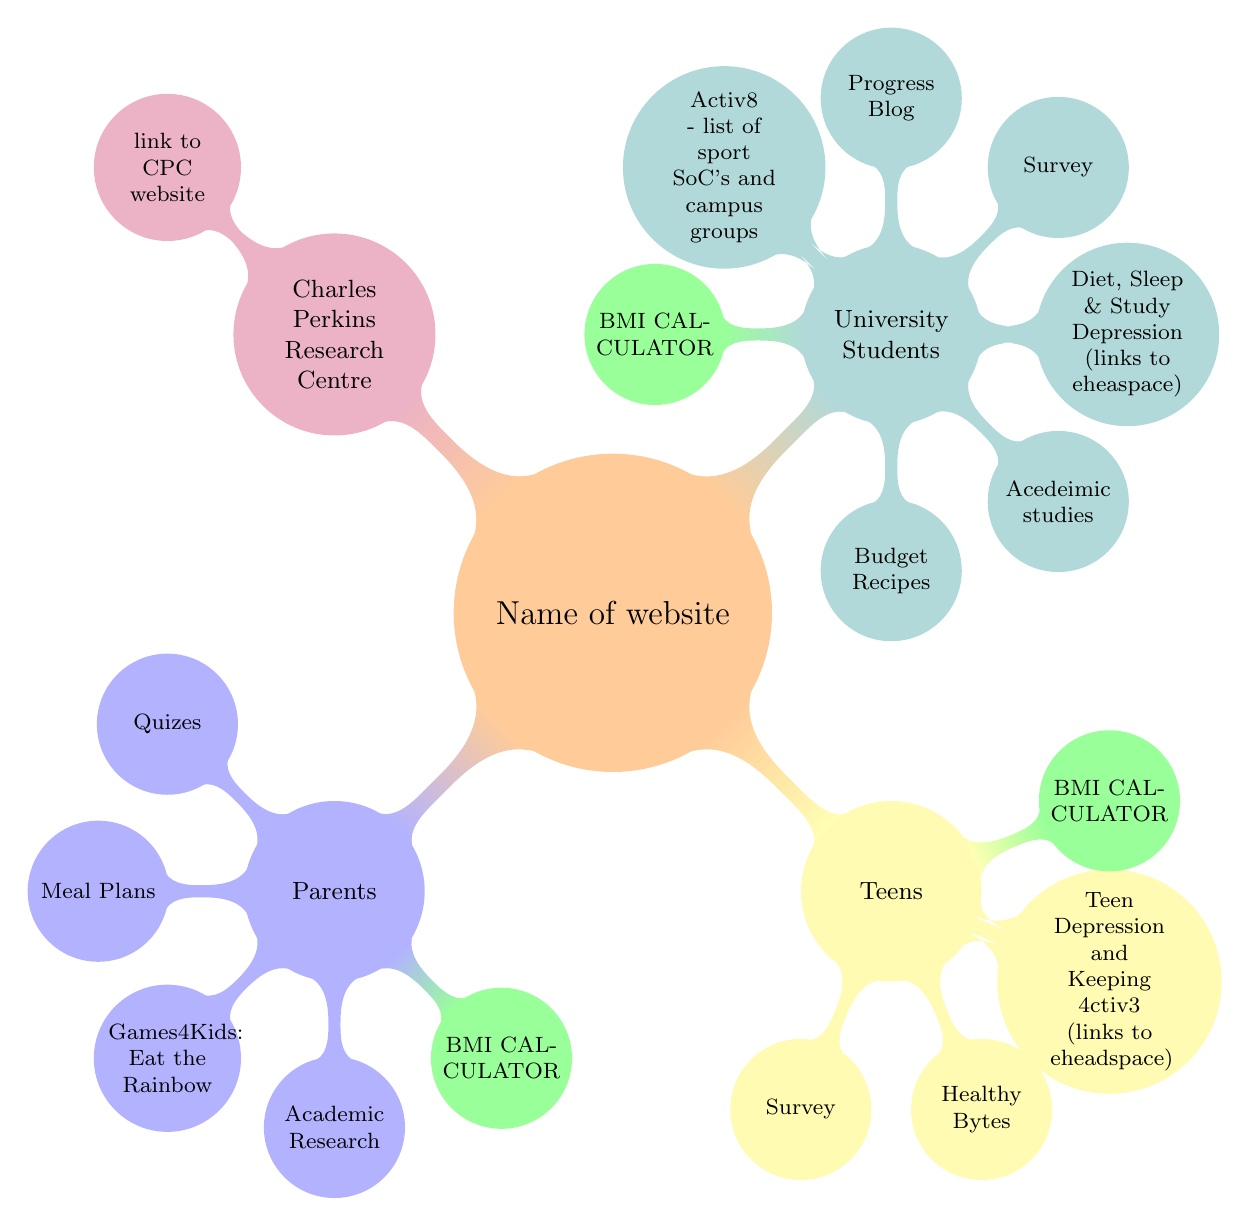
\begin{tikzpicture}[mindmap, grow cyclic, every node/.style=concept,
      concept color=orange!40,
      level 1/.append style={level distance=5cm,sibling angle=90},
      level 2/.append style={level distance=3cm,sibling angle=45},]
  %.
  \node{Name of website}
     child [concept color=blue!30] { node {Parents}
          child { node {Quizes}}
          child { node {Meal Plans}}
          child { node {Games4Kids: Eat the Rainbow}}
          child { node {Academic  Research}}
          child [concept color=green!40] { node {BMI CALCULATOR}}
      }
      child [concept color=yellow!30] { node {Teens}
          child { node {Survey}}
          child { node {Healthy Bytes}}
          child { node {Teen Depression and Keeping 4ctiv3 (links to eheadspace)}}
          child [concept color=green!40] { node {BMI CALCULATOR}}
      }
      child [concept color=teal!30] { node {University Students}
          child { node {Budget Recipes}}
          child { node {Acedeimic studies}}
          child { node {Diet, Sleep \& Study Depression (links to eheaspace)}}
          child { node {Survey}}
          child { node {Progress Blog}}
          child { node {Activ8 - list of sport SoC's and campus groups}}
          child [concept color=green!40] { node {BMI CALCULATOR}}
      }
      child [concept color=purple!30] { node {Charles Perkins Research Centre}
          child { node {link to CPC website}}
      };
  %.
  \end{tikzpicture}
  \caption{Sub-domain Hierarchy}
  \label{fig:subdomain-hierarchy}
\end{figure}

.
% include site_map.txt
%
% Copyright © 2014 Sara Lelliott. All Rights Reserved.
%
\begin{verbbox}

                                            +--------+ +------+   +--------+
                                            |register| |log in|   |site map|
                                            +--------+ +------+   +--------+



                                +-------------+
                                |contact us/  |
                                | credits     |
  +--------------------+        +---+---------+
  |                    |            |
  | home               +------------+--------------+
  |                    | +----------+-----+   +----+-----------+
  |                    | |about us/mission|   |CHARLES PERKINS |
  +-+-+------------+---+ | statement      |   | SITE           |
    | |            |     +-----+----------+   +----------------+
    | |            |
    | |            |
    | |   +--------v------+       +---------------+     +--------------+
    | |   |parents        +-------> BMI           +-----+ kids         |
    | |   +-----+---------+       +----+----------+     +----+---------+
    | |         |                      |                     |
    | |         |                      |                     |
    | |   +-----v--------+             |                     |
    | |   |meal plans    |       +-----v---------+    +------v-----------+
    | |   +-----+--------+       |quiz           |    | games            |
    | |         |                +---------------+    +------------------+
    | |   +-----+--------+
    | |   |blog          |
    | |   +--------------+
    | |
    | |
    | |
    | |
    | |
    | |  +--------------+      +----------+
    | +--+ teens        +------+ quizes   |
    |    +--------+-----+      +----------+
    |             |
    |             |           +--------------+
    |             +-----------+ BMI          |
    |                         | CALCULATOR   |
    |                         +--------------+
    |
    |
    |    +--------------+      +----------+
    +----+ uni students +------+ blog     |
         +---+----------+      +----------+
             |
             |           +--------------+
             +-----------+ BMI          |
                         | CALCULATOR   |
                         +--------------+

\end{verbbox}
\resizebox{0.95\textwidth}{!}{\theverbbox}


%% .. %%
\section{End User Types}
\subsection{Parents and Kids}

This page will consist of information on what childhood obesity is and contain statistics on how many Australian children are affected by this disease and other associated health risks. There will be a link to a BMI calculator, quizzes that parents can do with their child, an interactive game called "Eat the Rainbow", which encourages healthy food choices and pictures of physical activities that can be fun to encourage kids to play outside and develop positive habits to help them in later years. There will also be Information on developing healthy meal plans and recipes that cater to gluten free, dairy free, halal, kosher and vegan diets and a survey to ascertain qualitative data about the website.

%% .. %%
\subsection{Teens}

The Teen page will consist of photos of young people having fun out doors as well as fun indoors. There will also be links to "4ctiv3" a page of information on teen depression, connected to hormones and sleep patterns and not enough physical activity with links to eheadspace if further help is needed. There will be a links to a survey page to help collect data from the end user in order to verify whether this page is helpful and reaching the demographic, a function that could be added as an incentive, every x amount survey the user does they receive a \$10 Coles Myer gift voucher. There will be also a page called "Healthy Bytes" which has recipes for healthy snacks and exercises to do between online gaming sessions as poor eating habits can be developed at this time. There will also be a link to the BMI calculator.

%% .. %%
\subsection{University Students}

The main body of the University Student page will contain photos of young people outside at the beach, gym and studying. There will be information about why ample sleep and a balance diet is important to maintain health while studying. There will be a link called "Activat8" which will be a list of health/fittness SoCs and campus groups. There will be a link to a customisable progress blog where students can record there meals and cheat days and organise their diet and excercise. There will also be a link budget recipes so poor students won't have to resort to junk food to survive and a link to relevant acedemic studies on obesity and young adults. There will be a link to a survey to improve site functionality and BMI calculator.

%% .. %%
\section{Other Page Descriptions linked of the Main page}
\subsection{The Charles Perkins Centre}

The Charles Perkins Centre page will contain a brief description of who Charles Perkins was and what research is done there, also ther will be a link to the Charles Perkin's Centre website.

\subsection{Mission Statement} 

A page where we outline our core values and what we wish to achieve with this website and another list of useful links and related sources.


\subsection{About us}

About us will list the contributors to this website and contact.


%%%%%%%%%%%%%%%%
% End Document %
%%%%%%%%%%%%%%%%
\end{document}
%.
